\documentclass[10pt]{article}
\usepackage[margin=17mm]{geometry}
\usepackage{graphicx,booktabs,hyperref}
\usepackage[strings]{underscore}
\setlength{\parindent}{0pt}\setlength{\parskip}{5pt}
\begin{document}
\section*{Wide quartic constructor: instruction attribution}

Native retained runs, 2026-10-25; one before and one after, exact command
\texttt{ic_quartic_core_probe wide 6}. Frozen binaries:
before source 335d168aa, SHA prefix 81ab248653df; after source c46089aed,
SHA prefix df54670d4d21. AMD EPYC 9V74, Linux x86-64, shared managed host,
L0. Valgrind 3.24.0 Callgrind; one Rayon thread, no hardware PMU.

\begin{center}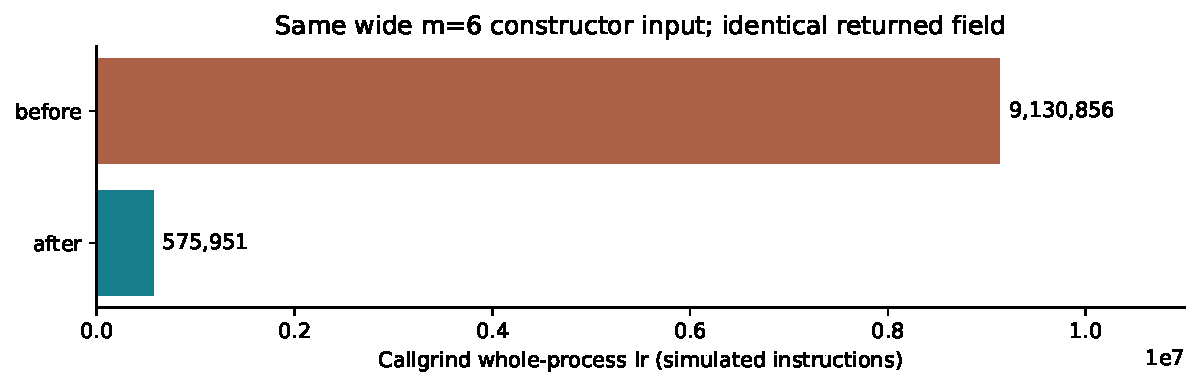
\includegraphics[width=\linewidth]{constructor-instructions.pdf}\end{center}
Measured simulated instruction totals are 9,130,856 and 575,951. A native
auditor independently parses raw summary/totals, matches hotspot JSON and
manifests, rehashes both frozen executables, and requires byte-identical
stdout. Both return base modulus 67 and extension coefficients [2,1,0,1].
Separate narrow/wide \texttt{both 6} controls also return identical output.

The implementation skips $X^4+c_1X+c_0$ when m is even and the perfect-fourth-
power case for every m. The readable exclusion is in CONSTRUCTOR_EXCLUSION.md;
six checked Lean dependencies include the conditional root-two-cycle theorem.
The finite-field/Frobenius/irreducibility bridge is not formalized. Identity
\texttt{IDC1h0e27b483c3989bcd} certifies the integer expansion only, with a faithful
Lean proof pointer; the v1 odd-prime evaluator is not a characteristic-two proof.

\begin{center}\begin{tabular}{rrl}\toprule
m & Base modulus (integer) & Extension coefficients $[c_0,c_1,c_2,c_3]$\\\midrule
16 & 69643 & [3, 1, 0, 1] \\
17 & 131081 & [1, 1, 0, 0] \\
18 & 262273 & [6, 1, 0, 1] \\
\bottomrule\end{tabular}\end{center}
All three separate field-constructor preflights exit zero under 12-GiB
address-space and 900-second limits. They establish representations only.

\textbf{Limits.} These instruction totals include loader/startup and the
Valgrind allocator. A/A repeats, five interleaved A/B rounds, the fastest
external field-constructor comparison and full-pipeline pricing are missing.
No native runtime, throughput, full-IC speedup or crossover is claimed.
The recorded profiler wall seconds are diagnostic and are not plotted.

\begin{flushleft}\footnotesize
Raw profiles:\par
\path{../../profiles/wide-constructor-before-20261025/}\par
\path{../../profiles/wide-constructor-after-20261025/}\par
Native audit:\par
\path{../../pipeline-receipts/wide-core-audit-20261025/constructor-profile-audit.json}\par
Protocols: WIDE_CONSTRUCTOR_PROFILE_PROTOCOL.md; WIDE_FIELD_CONSTRUCTOR_PROTOCOL.md;
WIDE_GROUP_AUDIT_PROTOCOL.md. Additional cloud VM allocation: none.
\end{flushleft}

\end{document}
